% chapters/chapter2/2_5_trajectory.tex
% !TeX root=../../main.tex

\section{برنامه‌ریز مسیر سینماتیکی}

یکی از چالش‌های بنیادین در کنترل سیستم‌های زیرفعال با محدودیت‌های سخت فیزیکی، نحوه اعمال موقعیت هدف به سیستم است. در معماری‌های پایه، معمولاً موقعیت نهایی به صورت یک ورودی پله (\lr{Step Input}) به سیستم اعمال می‌شود. اعمال یک‌باره خطای بزرگ موقعیت ($e = x_{ref} - x_0$) در لحظه شروع حرکت، کنترل‌کننده را وادار می‌کند تا برای کاهش سریع خطا، حداکثر نیروی ممکن را درخواست کند. این امر به صورت اجتناب‌ناپذیری به اشباع عملگرها (\lr{Actuator Saturation})، اعمال شوک‌های مکانیکی به سازه و نقض فرض‌های خطی‌سازی در زوایای کوچک می‌انجامد. در جابجایی‌های بزرگ، این رفتار خشن باعث خروج سریع آونگ از محدوده پایدار و بروز ناپایداری‌های فاز می‌شود.

برای غلبه بر این چالش ساختاری، لازم است موقعیت هدف نه به صورت یک جهش ناگهانی، بلکه در قالب یک مسیر پیوسته و سینماتیکی تولید شود. به همین منظور، از یک برنامه‌ریز مسیر (\lr{Trajectory Planner}) بر مبنای منحنی نرم (\lr{S-Curve}) استفاده می‌شود. این واحد با دریافت موقعیت اولیه و نهایی، یک پروفایل حرکتی مطلوب تولید می‌کند که در هر لحظه، مرجع موقعیت ($x_{ref}$)، سرعت ($\dot{x}_{ref}$) و شتاب ($\ddot{x}_{ref}$) را برای کالسکه تعیین می‌کند.

منطق ریاضی برنامه‌ریز مسیر بر پایه رعایت دقیق قیود سینماتیکی سیستم بنا شده است. این قیود شامل حداکثر سرعت مجاز کالسکه ($v_{\max}$) و حداکثر شتاب مجاز ($a_{\max}$) است که بر اساس ظرفیت نهایی موتورهای محرک و الزامات ایمنی جرثقیل تعیین می‌شوند. با استفاده از پروفایل \lr{S-Curve}، نرخ تغییرات شتاب (\lr{Jerk}) نیز محدود شده و انتقال حرکت کاملاً نرم و بدون ضربه صورت می‌پذیرد.

\begin{figure}[htbp]
    \centering
    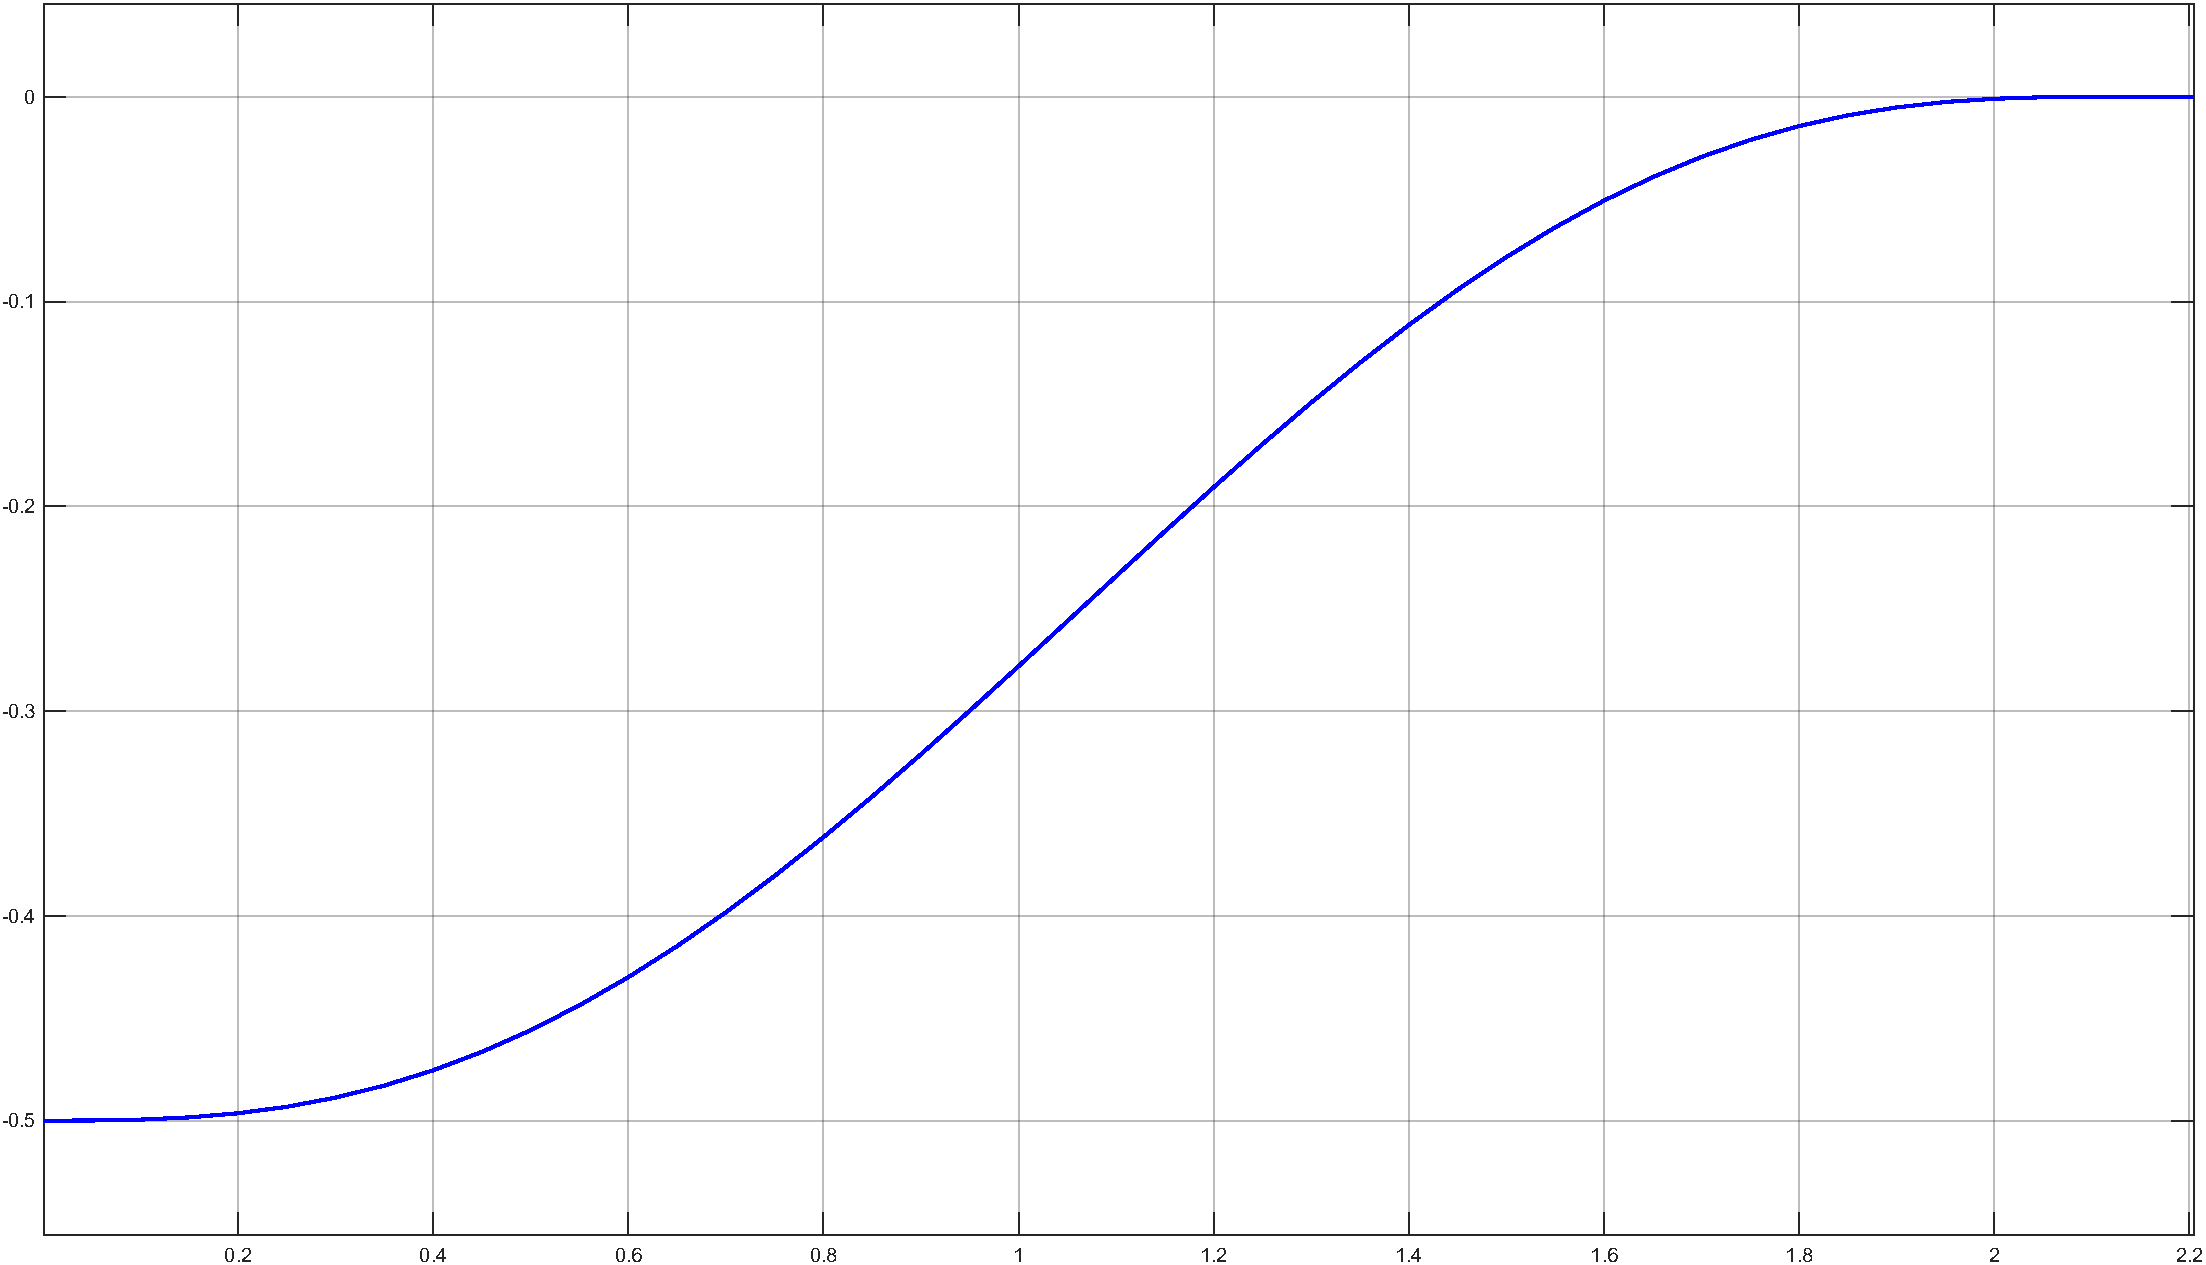
\includegraphics[width=0.8\textwidth]{images/4_NMPC_Trajectory/MPC_TRAJ_REF.pdf}
    \caption{نمونه‌ای از پروفایل مسیر مرجع نرم (\lr{S-Curve}) تولید شده توسط برنامه‌ریز سینماتیکی برای جابجایی ۰.۵ متر.}
    \label{fig:trajectory_ref}
\end{figure}

همان‌طور که در شکل \ref{fig:trajectory_ref} مشاهده می‌شود، با به‌کارگیری این برنامه‌ریز، خطای موقعیت در هر گام زمانی بسیار ناچیز و در محدوده خطی باقی می‌ماند. این پروفایل سینماتیکی به عنوان ورودی مرجع به سیستم کنترل تزریق می‌شود تا کالسکه با رعایت محدودیت‌های فیزیکی، به نرمی شتاب گرفته و در زمان مشخص به هدف برسد. در فصل‌های آتی، این مسیر مرجع به عنوان شالوده اصلی در طراحی کنترل‌کننده‌های ردیاب و پیش‌بین مورد استفاده قرار می‌گیرد.